\documentclass[11pt,a4paper]{article}
\usepackage[margin=2.3cm]{geometry}
\usepackage{amsmath,amssymb,amsthm,bm}
\usepackage{graphicx,booktabs,xcolor}
\usepackage[colorlinks=true,linkcolor=blue!60!black,urlcolor=blue!60!black]{hyperref}
\usepackage{caption}
\captionsetup{font=small,labelfont=bf}
\newtheorem{proposition}{Proposition}
\newtheorem{lemma}{Lemma}
\theoremstyle{remark}
\newtheorem{remark}{Remark}
\newcommand{\uu}{\bm{u}}
\newcommand{\ub}{\uu_b}
\newcommand{\nn}{\bm{n}}
\newcommand{\xx}{\bm{x}}
\newcommand{\Sf}{\bm{S}_f}
\newcommand{\Sw}{\bm{S}_w}
\newcommand{\Aw}{A_{\rm wall}}
\newcommand{\dd}{\,\mathrm{d}}
\newcommand{\code}[1]{\texttt{#1}}
\newcommand{\gradV}{\nabla_{\!V}}
\newcommand{\w}{\bm\omega}
\newcommand{\dt}{\Delta t}

\title{\bf Two open issues of the cut-cell IBM\\[3pt]
\large Rotating-wall mass source and second-order pressure gradient:\\
analysis, proposed fixes, verification plan}
\author{}
\date{\today}

\begin{document}
\maketitle

\noindent Notation as in \code{doc/cutCellIBM.pdf}: $\theta_f$ face and $\alpha_P$ cell fluid
fractions, $\Sf$ face area vector out of $P$, $\Sw=-\sum_f\theta_f\Sf$ the wall vector (from the
fluid into the body), $\Aw=|\Sw|$, $\nn_w=\Sw/\Aw$, $\xx_P$ cell centre, $\xx_c$ fluid centroid,
$\xx'_f$ wet-face centroid, $\ub(\xx)=\bm U+\w\times(\xx-\bm c)$ the rigid body velocity.
All numbers below are computed with the geometry algorithm of the library (bisection,
$32\times32$ sub-sampling, absorption below $\alpha_{\min}=0.02$) for a cylinder of radius $1$;
the scripts are next to this file.

\begin{table}[h]\centering\small
\begin{tabular}{@{}p{2.6cm}p{3.6cm}p{4.1cm}p{4.3cm}@{}}
\toprule
& branches & problem & proposed fix\\
\midrule
1.~rotating-wall mass source & \code{movingBody}, \code{scalar}; reduced on \code{scalar\_secondOrder}, \code{fouling}
& $S_P=\ub(\xx^e_P)\cdot\Sw$ is not zero for a wall moving tangentially: spurious local sources of
order $|\w|h\Aw$; with the centroid point also $\sum_PS_P\neq0$
& $S_P=\bm U\cdot\Sw+S^{\rm rot}_P$, the rotational part from the geometric wet faces;
exact flux through the discrete wall, $\sum_PS_P=0$ for any motion and mesh\\[3pt]
2.~second-order pressure gradient & \code{scalar\_secondOrder}, \code{fouling}
& face values sit at the centroid midpoint, $\theta_f=1$ faces are not corrected, the wall value
is at the normal foot of the centroid: errors of 17\% (median) in the cut cells for a linear $p$
& face correction relative to the centroid midpoint on every face of a cut cell; wall pressure
integrated over the wall pieces: exact for linear $p$\\
\bottomrule
\end{tabular}
\end{table}

\section{Issue 1: mass source of a rotating wall}

\subsection{What the code does}

For a moving body the continuity equation of a wall cell reads $\sum_f\phi_f=-S_P$ and the old
fluid fraction is recovered from the same source, $\alpha^n_PV_P=\alpha^{n+1}_PV_P-\dt S_P$. The
source is evaluated with the body velocity at one point per cell,
\begin{equation}
S_P=\ub(\xx^e_P)\cdot\Sw,\qquad
\xx^e_P=\begin{cases}
\xx_P+d_{\rm wall}\nn_w & \text{\code{movingBody}, \code{scalar}},\\
\xx_{c,P}+d_{\rm wall}\nn_w & \text{\code{scalar\_secondOrder}, \code{fouling}}.
\end{cases}
\label{eq:current}
\end{equation}
For a translation $\ub$ is uniform and \eqref{eq:current} is exact. For a rotation it is not.

\subsection{Why a point evaluation cannot work}

\begin{lemma}
\label{lem:normal}
For a rigid velocity and any $s$, $\ub(\xx+s\nn_w)\cdot\nn_w=\ub(\xx)\cdot\nn_w$.
\end{lemma}
\begin{proof}
$(\w\times s\nn_w)\cdot\nn_w=0$.
\end{proof}

\begin{lemma}
\label{lem:planar}
For a planar surface $\Gamma$ with area vector $\bm S_\Gamma$ and centroid $\xx_\Gamma$,
$\int_\Gamma\ub\cdot\nn\dd S=\ub(\xx_\Gamma)\cdot\bm S_\Gamma$.
\end{lemma}
\begin{proof}
$\ub$ is linear in $\xx$ and $\nn$ is constant on $\Gamma$.
\end{proof}

In two dimensions the wall of a cut cell is the chord between the two edge crossings, and $\Sw$
is normal to it. For a body of revolution rotating about its axis, the chord midpoint $\xx_m$
lies on the line through the centre along $\Sw$, so $\ub(\xx_m)\cdot\Sw=0$: the exact flux
through the discrete wall vanishes, as it must, since the geometry does not change. A point
evaluation gives instead
\begin{equation}
S_P=\ub(\xx^e_P)\cdot\Sw=\big(\w\times(\xx^e_P-\xx_m)\big)\cdot\Sw
=\w\cdot\big((\xx^e_P-\xx_m)\times\Sw\big),
\end{equation}
which depends only on the offset of $\xx^e_P$ \emph{across} the normal (Lemma~\ref{lem:normal}).
The cell centre is offset by $O(h)$, so $|S_P|=O(|\w|h\Aw)$ with alternating sign around the body.
Moving the point along $\nn_w$, as on \code{movingBody} and \code{scalar}, changes nothing:
Fig.~\ref{fig:source}b shows the two forms coincide to round-off. The centroid of
\code{scalar\_secondOrder} is not on the line either, and the spurious source is of the same size
(Fig.~\ref{fig:source}b); in the Taylor--Couette case it happened to be smaller than with the
cell centre.

\begin{figure}[h]\centering
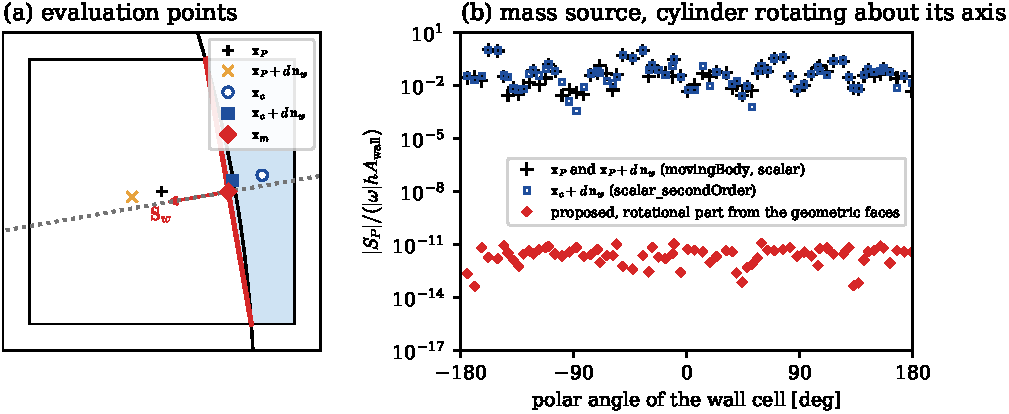
\includegraphics[width=\textwidth]{h_source.pdf}
\caption{(a)~A cut cell of a cylinder rotating about its axis (dotted: the line through the centre
along $\Sw$). $\xx_P$ and $\xx_P+d\nn_w$ lie on a common normal and give the same source; only
points on the dotted line, such as the chord midpoint $\xx_m$, give zero. (b)~Source of every wall
cell for $\w=1$, $h=0.1$, normalised with $|\w|h\Aw$.}
\label{fig:source}
\end{figure}

\paragraph{Consequences.}
(i)~A body rotating in place has static geometry, yet the solver assigns $\alpha^n_P\neq
\alpha^{n+1}_P$ and a non-zero divergence to its wall cells; the resulting local sources
checkerboard the cut-cell pressure (errors of $\pm0.4$ in the Taylor--Couette case before the
centroid evaluation, for a pressure range of $0.08$).
(ii)~Compatibility. Since $\sum_P\bm S_{w,P}=\bm 0$ for a closed body,
\begin{equation}
\sum_PS_P=\w\cdot\sum_P\xx^e_P\times\bm S_{w,P}
=\w\cdot\sum_{f}\theta_f\,(\xx^e_N-\xx^e_O)\times\Sf .
\label{eq:sum}
\end{equation}
With $\xx^e=\xx_P+d\nn_w$ this is the cell-centre form, $\bm d_f\times\Sf$, which vanishes on
orthogonal meshes. With the centroid it does not vanish: for the cylinder of
Fig.~\ref{fig:source} $\sum_PS_P=-1.2\times10^{-3}$, against individual sources of
$10^{-2}$. By the reference lemma of \code{cutCellIBM.pdf} (Lemma~1) this defect is deposited at
the pressure reference cell as a point source. The Taylor--Couette case logged $10^{-17}$ only
because its geometry is mirror-symmetric.

\subsection{Proposed fix}

Split the motion into the translation of the reference point $\bm c$ and the rotation about it.
The translational part is kept as it is, because it is what makes free-stream preservation exact
(it includes the faces closed by sliver absorption, which carry the swept volume of the absorbed
cell). The rotational part is computed as a flux through the geometric wall. Since
$\w\times(\xx-\bm c)$ is divergence-free and linear, the divergence theorem over the geometric
fluid polygon $\Omega^{\rm geo}_P$ of cell $P$ (bounded by the wet faces before any
post-processing and by the chord) gives exactly
\begin{equation}
S^{\rm geo}_P\equiv\int_{\text{chord}}\big(\w\times(\xx-\bm c)\big)\cdot\nn\dd S
=-\sum_{f\in P}\theta^{\rm geo}_f\,\big(\w\times(\xx'^{\rm geo}_f-\bm c)\big)\cdot\Sf ,
\label{eq:Sgeo}
\end{equation}
with $\theta^{\rm geo}_f$ and $\xx'^{\rm geo}_f$ the fraction and wet-face centroid of the face
\emph{before} absorption and synchronisation (a face value of a linear field over a planar face
is the value at its centroid). Cells removed by the post-processing (absorbed slivers, and cells
with $\alpha=0$ from the sampling but wet faces) form the set $\mathcal R$; their $S^{\rm geo}$ is
handed to their fluid face neighbours in proportion to the shared geometric wet area. The
proposed source is
\begin{equation}
\boxed{\;S_P=\bm U\cdot\bm S_{w,P}+S^{\rm geo}_P+\sum_{N\in\mathcal R,\,N\sim P}w_{NP}\,S^{\rm geo}_N,
\qquad w_{NP}=\frac{\theta^{\rm geo}_{f_{NP}}|\bm S_{f_{NP}}|}
{\sum_{f\in N,\ \text{other side fluid}}\theta^{\rm geo}_f|\Sf|}\;}
\label{eq:new}
\end{equation}

\begin{proposition}
\label{prop:source}
The source \eqref{eq:new} has the following properties.
\begin{enumerate}\itemsep1pt
\item \emph{Translation unchanged.} For $\w=\bm 0$ it is the current source; free-stream
      preservation (Proposition~7 of \code{cutCellIBM.pdf}) is unaffected.
\item \emph{Exact flux through the discrete wall.} Outside the neighbourhood of $\mathcal R$ the
      rotational part is the exact flux of the rotation through the chord(s) of the cell. For a
      body of revolution rotating about its axis it vanishes in two dimensions (to the bisection
      tolerance), so a body rotating in place has $S_P=0$ and $\alpha^n_P=\alpha^{n+1}_P$.
\item \emph{Compatibility for every rigid motion and every mesh.}
      $\sum_PS_P=\bm U\cdot\sum_P\bm S_{w,P}-\sum_{\rm all\ cells}\sum_{f}\theta^{\rm geo}_f
      \big(\w\times(\xx'^{\rm geo}_f-\bm c)\big)\cdot\Sf=0$: the handover conserves
      $\sum S^{\rm geo}$, and every internal face appears twice with the same $\theta^{\rm geo}_f$
      and $\xx'^{\rm geo}_f$ and opposite $\Sf$. On periodic faces the two copies are mapped to
      the same minimum image about $\bm c$ and cancel as well.
\end{enumerate}
\end{proposition}

\noindent Numerically (Fig.~\ref{fig:source}b, $h=0.1$, 7 cells in $\mathcal R$): $\max_P|S_P|=7\times
10^{-14}$ for the rotation about the axis (against $1.1\times10^{-2}$ today), and $\sum_PS_P=
6\times10^{-17}$ also for an eccentric rotation ($\bm c=(0.3,-0.2)$), where the centroid form
gives $-1.2\times10^{-3}$.

\begin{remark}
In three dimensions the chord becomes the wall polygon of the cut cell; \eqref{eq:Sgeo} is then the
flux through the polyhedral approximation of the surface, which is not exactly zero for a
sphere rotating about a diameter but converges to zero with the geometry. Properties 1 and 3 hold
unchanged.
\end{remark}

\begin{remark}
The point $\xx^e_P$ is still needed for the \emph{tangential} wall velocity of the no-slip
traction $\nu\Aw(\uu_P-\ub)/d$. There the current choices are appropriate: the value at the
foot of the normal from the location of the cell value, $\xx_P+d\nn_w$ (first order) or
$\xx_c+d_c\nn_w$ (second order), is what the two-point wall gradient differences against. Only
the mass source changes.
\end{remark}

\paragraph{Implementation.}
\begin{itemize}\itemsep1pt
\item \code{faceFractions}: keep $\theta^{\rm geo}_f$ and the wet-face centroid of every face as
      computed, before absorption and synchronisation (\code{scalar\_secondOrder} already
      computes the wet-face offset; \code{movingBody}/\code{scalar} need the few lines of the
      fan-triangulated centroid).
\item \code{bodyMotion}/\code{ibmBody}: accessors for $\bm U$, $\w$ and the current centre
      $\bm c(t)$, and the minimum-image map already used for the level set.
\item \code{calcMovingTerms}: $S_P=\bm U_{b(P)}\cdot\Sw$ as now, plus a loop over the faces for
      \eqref{eq:Sgeo} and the handover of $\mathcal R$ (across processor faces with
      \code{syncTools}). $\alpha^n$ follows from $S_P$ as now. Cost: one face loop per step.
\item Cells shared by two bodies: use the body of the cell, as now; faces between cells of two
      different moving bodies are the one remaining case where $\sum_PS_P$ is not exact.
\end{itemize}

\paragraph{Verification.}
\begin{enumerate}\itemsep1pt
\item Cylinder rotating in place (\code{motion \{type none; angularVelocity (0 0 1);\}}):
      $\max_P|S_P|$ at round-off, $\alpha^n=\alpha^{n+1}$, no checkerboard in the cut-cell
      pressure.
\item Taylor--Couette (\code{tutorials/order/taylorCouette}) on all moving branches, first- and
      second-order: velocity and pressure errors against the current ones.
\item Eccentric rotation or a rotating ellipse: $\sum_PS_P$ at round-off.
\item Regression: free stream, oscillating and translating cylinder must be bit-identical
      (pure translation).
\end{enumerate}

\section{Issue 2: second-order pressure gradient}

\subsection{What the code does}

With \code{secondOrder true} the volume-integrated gradient is
\begin{equation}
\gradV p\big|_P=\sum_f\theta_f\Big[\bar p_f+[0<\theta_f<1]\,\bm g_f\cdot(\xx'_f-\xx_f)\Big]\Sf
+\big[p_P+d\,\bm g_P\cdot\nn_w\big]\Sw ,
\label{eq:grad2}
\end{equation}
with $\bar p_f=w_fp_O+(1-w_f)p_N$ the linear interpolate, $\bm g$ the least-squares gradient on
the centroids ($\bm g_f$ its face average) and $d$ the centroid wall distance. The comment in the
code and the methods document before its revision stated that this is exact for a linear pressure.

\subsection{Why it is not exact}

Take $p=p_0+\bm G\cdot\xx$ with cell values at the centroids, $p_P=p(\xx_{c,P})$; the
least-squares gradient is then exact, $\bm g=\bm G$. The exact integral over the geometric fluid
polygon is $\oint p\,\nn\dd S=V^{\rm geo}_P\bm G$. Three terms of \eqref{eq:grad2} miss it:
\begin{enumerate}\itemsep1pt
\item The linear interpolate is the value at the weighted midpoint of the two \emph{centroids},
      $\bar p_f=p(\bm m_f)$, $\bm m_f=w_f\xx_{c,O}+(1-w_f)\xx_{c,N}$, not at the face centre. The
      correction $\bm G\cdot(\xx'_f-\xx_f)$ therefore leaves the error $\bm G\cdot(\bm m_f-\xx_f)$,
      i.e.\ $\tfrac12\bm G\cdot(\bm o_O+\bm o_N)$ on a uniform mesh, on every partially wet face.
\item Faces with $\theta_f=1$ next to a cut cell are not corrected at all, although
      $\bm m_f\neq\xx_f$ there.
\item The wall value is taken at $\xx_c+d\nn_w$, the normal foot of the centroid, while the exact
      integral over a planar wall is the value at the wall centroid $\xx_m$ (Lemma~\ref{lem:planar}
      with $p$ for $\ub$). The tangential offset gives $\bm G\cdot(\xx_c+d\nn_w-\xx_m)\,\Sw$; for a
      cell next to an absorbed sliver or a staircase face the wall is not even planar.
\end{enumerate}
Fig.~\ref{fig:grad}b shows the result: relative errors of $0.17$ (median) and up to $5.7$ in the
cut cells, not better than the first-order form ($0.28$ and $6.5$).

\subsection{Proposed fix}

\begin{equation}
\bar p_f\;\to\;\bar p_f+\bm g_f\cdot(\xx'_f-\bm m_f)\qquad\text{on every open face of a cell with
}\bm o\neq\bm 0\text{ or }\theta_f<1,
\label{eq:face}
\end{equation}
\begin{equation}
p_P\Sw\;\to\;\sum_k\big[p_P+\bm g_P\cdot(\xx_k-\xx_{c,P})\big]\bm S_k ,
\label{eq:wall}
\end{equation}
where the wall of the cell is split into pieces $k$ with area vectors $\bm S_k$ and centroids
$\xx_k$ (Fig.~\ref{fig:grad}a): the chord(s) of the geometric cut (midpoint), and every
geometrically wet part of a face that the post-processing closed (area vector
$\theta^{\rm geo}_f\Sf$, centroid $\xx'^{\rm geo}_f$). By the closure of the geometric polygon,
$\sum_k\bm S_k=\Sw$. On faces between two full cells of an orthogonal mesh $\bm m_f=\xx'_f=\xx_f$
and \eqref{eq:face} is zero, so the uncut part of the domain is untouched.

\begin{proposition}
\label{prop:grad}
If the least-squares gradient is exact for linear fields, the gradient with \eqref{eq:face} and
\eqref{eq:wall} satisfies $\gradV p|_P=V^{\rm geo}_P\bm G$ for every linear $p$ and every wall cell.
It vanishes for a uniform $p$, conserves momentum (the face corrections are antisymmetric, since
$\xx'_f$ and $\bm m_f$ are shared by both cells), and the pressure force
$\bm F_p=\sum_P\sum_kp_k\bm S_k$ keeps the momentum-sum identity.
\end{proposition}
\begin{proof}
Each face term equals $p(\xx'_f)\theta_f|\Sf|\,\nn_f$, the exact integral over the wet face; each
wall term equals $p(\xx_k)\bm S_k$, the exact integral over the planar piece $k$. Together the wet
faces and the pieces are the boundary of $\Omega^{\rm geo}_P$, and the divergence theorem gives
$V^{\rm geo}_P\bm G$. For uniform $p$ the sum is $p(\sum_f\theta_f\Sf+\sum_k\bm S_k)=\bm 0$.
\end{proof}

\noindent Numerically: over 880 wall cells (12 mesh offsets) the relative error is below
$4\times10^{-13}$ (Fig.~\ref{fig:grad}b). The wall distance $d$ is no longer needed in the
gradient.

\begin{figure}[h]\centering
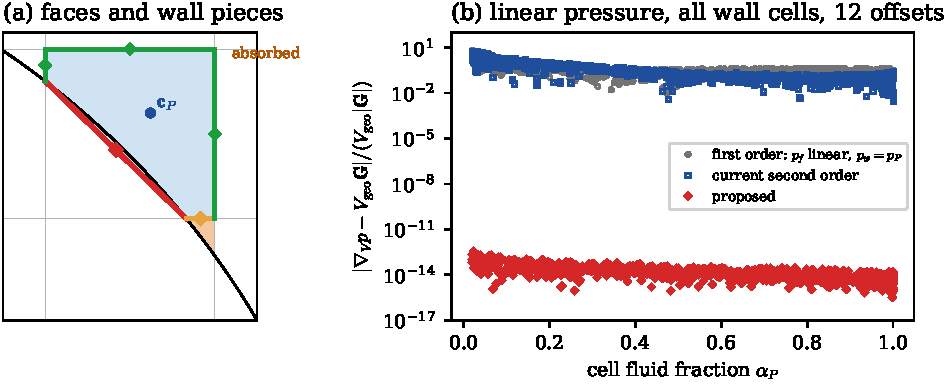
\includegraphics[width=\textwidth]{h_grad.pdf}
\caption{(a)~A cell next to an absorbed sliver: open wet faces with their centroids (green), the
chord with its midpoint (red) and the wet part of the face closed by the absorption (orange); the
last two are the wall pieces of \eqref{eq:wall}. (b)~Relative error of the cut-cell gradient of a
linear pressure against the exact integral over the geometric polygon.}
\label{fig:grad}
\end{figure}

\begin{remark}
In three dimensions the chord is the wall polygon formed by the crossings of the cell's cut edges
(each cut face contributes one segment); its centroid by fan triangulation makes \eqref{eq:wall}
exact for planar cuts and second-order accurate otherwise.
\end{remark}

\begin{remark}[What the fix does not do]
It makes the gradient consistent; it does not change the conditioning of the cut-cell pressure
rows (the mobility of a cut cell still scales with its fluid fraction, Section~8.6 of
\code{cutCellIBM.pdf}). How much of the non-convergence of the cut-cell pressure in the
Taylor--Couette case is due to the gradient and how much to the conditioning is exactly what the
re-run will tell; cell merging remains the remedy for the latter.
\end{remark}

\begin{remark}[Hydrostatic balance]
A fluid at rest under a uniform body force $\bm g$ in a closed domain has $p=\bm g\cdot\xx$. With
the fix the pressure force of a cut cell is $V^{\rm geo}_P\bm g$, the body force $\alpha_PV_P\bm
g$; the residual $(\alpha_PV_P-V^{\rm geo}_P)\bm g$ is the sub-sampling error of $\alpha$
($\sim10^{-3}$). Weighting the body force with the polygon volume (or computing $\alpha$ from the
polygon, exact in two dimensions) would make the scheme exactly well balanced.
\end{remark}

\paragraph{Implementation.}
\begin{itemize}\itemsep1pt
\item \code{calcGeometry} (second-order path): store per wall cell the list of wall pieces
      (chords from the cut edges of the cell, closed geometric wet parts from the faces with
      $\theta_f=0<\theta^{\rm geo}_f$) and $\bm m_f$ per face from \code{mesh.weights()} and the
      centroid offsets.
\item \code{grad()}: replace the face correction by \eqref{eq:face} on every open face touching
      a cell with a non-zero offset, and the wall term by \eqref{eq:wall}; \code{forces()} uses
      the same pieces.
\end{itemize}

\paragraph{Verification.}
\begin{enumerate}\itemsep1pt
\item \code{ibmOrderTest}: new problems for the gradient operator alone --- linear $p$ (error at
      the sub-sampling level of $V^{\rm geo}$ vs $\alpha V$) and quadratic $p$ (second order in
      the cut cells).
\item Hydrostatic box with an immersed body: spurious velocity against the current scheme.
\item Taylor--Couette pressure errors and the drag Richardson study, with the components.
\end{enumerate}

\section{Suggested order}

\begin{enumerate}\itemsep1pt
\item Issue 1 on \code{movingBody} (about one day with tests), merged into \code{scalar},
      \code{scalar\_secondOrder} (where it replaces the centroid evaluation of the source) and
      \code{fouling}.
\item Issue 2 on \code{scalar\_secondOrder} (one to two days, three-dimensional wall polygons
      included), merged into \code{fouling}; then re-run Taylor--Couette and the drag study
      with both fixes, and update \code{doc/cutCellIBM.tex} and \code{doc/secondOrderStudy.md}.
\end{enumerate}

\end{document}
